\documentclass{beamer}
%Information
\title{Algebra 1: Quadratic Equation and Linear Equation}
\titlegraphic{\hfill
\includegraphics[height=1cm]{orange.png}}
\institute{Youth STEM Academy}
\author{Erzhuo Wang}
\date{July 10,2024}
%Theme
\usetheme[block=fill, sectionpage=none]{metropolis}
\useoutertheme{infolines}
\useinnertheme{metropolis}
\setbeamertemplate{blocks}[rounded][shadow=false]
\setbeamertemplate{items}[ball]
\setbeamertemplate{sections/subsections in toc}[ball]
\setbeamertemplate{headline}{}
\logo{YSA}
\usecolortheme{custom}
%\usetheme{Madrid}
%\usetheme{Heverlee}

%Setting
\usepackage[UTF8,noindent]{ctexcap}
\theoremstyle{definition}
\newtheorem{defn}{Definition}[section]
\newtheorem{coro}[defn]{Corollary}
\newtheorem{theo}[defn]{Theorem}
\newtheorem{exer}[defn]{Exercise}
\newtheorem{rema}[defn]{Remark}
\newtheorem{lem}[defn]{Lemma}
\newtheorem{prop}[defn]{Proposition}
\newtheorem{nota}[defn]{Notation}
\newtheorem{exam}[defn]{Example}
\newtheorem{ques}[defn]{Question}

\newenvironment{prooff}{{\noindent\it\textcolor{cyan!40!black}{Proof}:}\,}{\par}
\newenvironment{proofff}{{\noindent\it\textcolor{cyan!40!black}{Proof of the lemma}:}\,}{\qed \par}
\newcommand{\bbrace}[1]{\left\{ #1 \right\} }
\newcommand{\bb}[1]{\mathbb{#1}}
\newcommand{\p}{^{\prime}}
\renewcommand{\mod}[1]{(\text{mod}\,#1)}
\newcommand{\blue}[1]{\textcolor{blue}{#1}}
\newcommand{\spec}[1]{\text{Spec}({#1})}
\newcommand{\rarr}[1]{\xrightarrow{#1}}
\newcommand{\larr}[1]{\xleftarrow{#1}}
\newcommand{\emptyy}{\underline{\quad}}
\newenvironment{enu}{\begin{enumerate}[(1)]}{\end{enumerate}}
%ctrl+点击文本返回代码  选中代码 ctrl+alt+j 为代码查找文本
\begin{document}
\begin{frame}
    \titlepage
\end{frame}
\begin{frame}{Introduction}
    本节课我们学习如何解一元二次方程和一个二元一次方程组, 在实际解题过程中我们需要对题目所描述的实际问题进行建模, 然后去求解.
\end{frame}
\begin{frame}{Linear Euqation}
    \begin{exam}
        解下面的方程:
    $$ 
        \begin{cases}
                x+3y=5 \\ 
                2x-7y=3           
        \end{cases}
    $$
    \end{exam}
    我们一般采用消元法消去其中一个未知数, 从而得到另一个两个未知数的具体取值.
\end{frame}
\begin{frame}{Frog}
    A group of frogs (called an army) is living in a tree. A frog turns green when in the shade and turns yellow when in the sun. 
    Initially, the ratio of green to yellow frogs was $3: 1$. Then 3 green frogs moved to the sunny side and 5 yellow frogs moved to the shady side. 
    Now the ratio is $4: 1$. What is the difference between the number of green frogs and the number of yellow frogs now?

    (A) 10 (B) 12 (C) 16 (D) 20 (E) 24
\end{frame}
\begin{frame}{Rectangles(AMC 8, 2020-25)}
    $S_1,S_2,S_3$为三个正方形, 大矩形长$3322$, 宽$2020$, 求$S_2$边长($S_1$和$S_3$边长不一定相等).
    \begin{figure}
        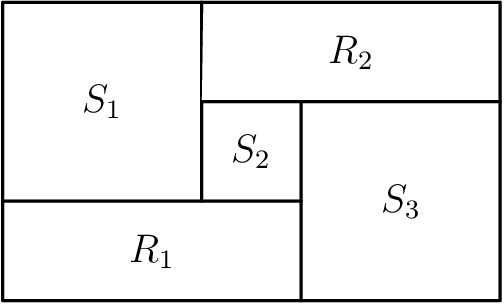
\includegraphics[height=0.4\textheight]{rectangle1.png}
    \end{figure}
\end{frame}
% \begin{frame}{Some Set Theory Prerequisites(一些集合论前置)}
%     \begin{exam}
%         Some examples of set: $\mathbb{Z}$(all the integers), $\mathbb{Q}$(all the rational integers), $\mathcal{P}$(all the prime number).
%     \end{exam}
%     \begin{defn}
%         If $a$ is an element of $A$, we denote it $a\in A$.
%     \end{defn}
%     \begin{defn}
%         If $f:A\rightarrow B$ is a map, $f$ is injective if $x\neq y$ implies $f(x)\neq f(y)$.

%         $f$ is surjective if for all $b\in B$, there's $a\in A$ such that $f(a)=b$.
%     \end{defn}
%     \begin{defn}
%         If $A$, $B$ are sets, we denote the intersection of $A$ and $B$ by $A\cap B$. The union of $A$ and $B$ by $A\cup B$.
%     \end{defn}
% \end{frame}
% \begin{frame}{History of Number System(数系扩张历史)}
%     \begin{equation*}
%         \mathbb{Z}\hookrightarrow \mathbb{Q} \hookrightarrow \mathbb{R} (\hookrightarrow \bar{\bb{Q}}\hookrightarrow)\mathbb{C}
%     \end{equation*}
%     古希腊时期,为了找出直角边为$1$的等腰直角三角形的斜边长, 人们创造出了无理数(Irrational Number), 无理数和有理数组成实数.

%     后来, 为了解方程
%     \begin{equation*}
%         x^2+1=0
%     \end{equation*}
%     人们创造出了复数(Complex Number). 再后来人们发现,
%     复数中有些数是整系数多项式方程的根, 而有些数不是(比如$\pi$), 这又诱导了代数数$\bar{\bb{Q}}$(Algebraic Number)和超越数概念的出现.

%     对代数数的研究是现代数论的核心, 为此, 数学家们创造了数不尽的理论.

% \end{frame}
% \begin{frame}{Quadratic Formula}
%     When $a, b$, and $c$ are real numbers, the quadratic equation $a x^2+b x+c=0$ with discriminant $D=$ $b^2-4 a c$ has
%     two solutions
%     \begin{enu}
%         \item two distinct real numbers when $D>0$,
%         \item two equal real numbers when $D=0$, and
%         \item no real solution when $D<0$.
%     \end{enu}
%     \begin{theo}[Quadratic Formula]
%         For real number $a,b$ and $c$, the two solutions to the quadratic equation $ax^2+bx+c=0$ is given the quadratic formula
%         \begin{equation*}
%             x=\frac{-b\pm \sqrt{b^2-4ac}}{2a}
%         \end{equation*}
%     \end{theo}
% \end{frame}
\begin{frame}{二次方程求根公式}
    当$a,b,c$为实数时, 记二次方程$ax^2+bx+c=0,a\neq 0$的判别式为$D=b^2-4ac$
    \begin{enu}
        \item $D>0$时, 有两个不同的实数解.
        \item $D=0$时, 只有一个实数解.
        \item $D<0$时,   没有实数解.
    \end{enu}
    \begin{theo}[Quadratic Formula]
        $D>0$时候, 二次方程$ax^2+bx+c=0,a\neq 0$的解由如下公式给出:
        \begin{equation*}
            x=\frac{-b\pm \sqrt{b^2-4ac}}{2a}
        \end{equation*}
    \end{theo}
\end{frame}

% \begin{frame}{Polynomials}
%     A polynomial is of the form
%     $$
%         a_n x^n+a_{n-1} x^{n-1}+a_{n-2} x^{n-2}+\cdots+a_1 x+a_{01}
%     $$
%     where $a_n \neq 0$ is the leading coefficient. If $a_n=1$, then the polynomial is called monic. $a_0$ is the constant term, and $n$ is the degree of this polynomial. Usually, we
%     denote the set of polynomials with real number coefficient by $\bb{R}[x]$.

%     For a polynomial function
%     $$
%         p(x)=a_n x^n+a_{n-1} x^{n-1}+a_{n-2} x^{n-2}+\cdots+a_1 x+a_0
%     $$
%     if a number c satisfies $p(c)=0$, then $c$ is a root (sometimes called a zero) of $p(x)$.
% \end{frame}
% \begin{frame}{Factorization in $\bb{R}[x]$}
%     \begin{defn}
%         $d(x)$ divides(整除) $f(x)$ if there's $g(x)\in \bb{R}[x]$ such that $d(x)g(x)=f(x)$. And if $d(x)$ divides $f(x)$, we
%         call $d(x)$ a factor(因子) of $f(x)$.
%     \end{defn}
%     \begin{theo}
%         If real number $c$ is a root of $f(x)$, then $x-c$ is a factor of $f(x)$.
%     \end{theo}
%     \begin{defn}
%         $p(x)$(degree $\ge 1$) is a irreducible polynomial if there's no polynomial $d(x)$ with degree $\ge 1$ such that
%         $d(x)|p(x)$ and $d(x)\neq cp(x)$, where $c$ is a non-zero real number.

%     \end{defn}
% \end{frame}
% \begin{frame}{Classical Formula}
%     Assume that $a, b$, and $c$ are constants and $n$ is a positive integer. Then
%     $$
%         \begin{aligned}
%             a x^2+b x       & =x(a x+b)                                                                       \\
%             x^2+(b+c) x+b c & =(x+b)(x+c)                                                                     \\
%             x^2+2 a x+a^2   & =(x+a)^2                                                                        \\
%             x^2-a^2         & =(x-a)(x+a)                                                                     \\
%             x^3-a^3         & =(x-a)\left(x^2+a x+a^2\right)                                                  \\
%             x^3+a^3         & =(x+a)\left(x^2-a x+a^2\right)                                                  \\
%             x^n-a^n         & =(x-a)\left(x^{n-1}+x^{n-2} a+x^{n-3} a^2+\cdots+a^{n-1}\right)                 \\
%             x^n+a^n         & =(x+a)\left(x^{n-1}-x^{n-2} a+x^{n-3} a^2-\cdots+a^{n-1}\right), n \text{ odd}.
%         \end{aligned}
%     $$
% \end{frame}
\begin{frame}{Vieta's Theorem}
    \begin{theo}[Vieta's Theorem for quadratic polynomials]
        If $x_1$ and $x_2$ are two roots of the quadratic polynomial $ax^2+bx+c$, we have
        \begin{equation*}
            x_1+x_2=-\frac{b}{a}, x_1x_2=\frac{c}{a}
        \end{equation*}
    \end{theo}
    \begin{exam}
        Assume $\alpha$ and $\beta$ are two roots of the equation $2x^2+x-7=0$. Find
        \begin{equation*}
            \alpha^2+\beta^2, \frac{1}{\alpha}+\frac{1}{\beta}, \alpha^3+\beta^3
        \end{equation*}
    \end{exam}
\end{frame}
\begin{frame}{Vieta's Theorem(韦达定理)}
    \begin{theo}[Vieta's Theorem for quadratic polynomials]
        如果$x_1$和$x_2$是二次方程$ax^2+bx+c=0$的两个根,我们有
        \begin{equation*}
            x_1+x_2=-\frac{b}{a}, x_1x_2=\frac{c}{a}
        \end{equation*}
    \end{theo}
    \begin{exam}
        Assume $\alpha$ and $\beta$ are two roots of the equation $2x^2+x-7=0$. Find
        \begin{equation*}
            \alpha^2+\beta^2, \frac{1}{\alpha}+\frac{1}{\beta}
        \end{equation*}
    \end{exam}
\end{frame}
\begin{frame}{Exercise}
    \begin{ques}
        Suppose that the equation $x^2-px+q=0$ has solutions $x=a$ and $y=b$. What's the equations
        has solutions $x=a+\frac{1}{b}$ and $x=b+\frac{1}{a}$.
    \end{ques}
    % \begin{ques}
    %     Factor each of the following polynomial:
    %     \begin{equation*}
    %         x^2+15x+36
    %     \end{equation*}
    %     \begin{equation*}
    %         x^3+5^3
    %     \end{equation*}
    %     \begin{equation*}
    %         x^3-6x^2+11x-6
    %     \end{equation*}
    % \end{ques}
\end{frame}
\begin{frame}{Exercise}
    \begin{ques}[AMC 8, 2019-20]
        How many different real numbers $x$ satisfy the equation

        有多少不同的实数x满足这个方程
        \begin{equation*}
            (x^2-5)^2=16
        \end{equation*}
    \end{ques}
\end{frame}
\begin{frame}{Gray Square Tiles(AMC 8, 2020-24)}
    A large square region is paved with $n^2$ gray square tiles, each measuring $s$ inches on a side. A border $d$ inches wide surrounds each tile. The figure below shows the case for $n=3$. When $n=24$, the 576 gray tiles cover $64 \%$ of the area of the large square region. What is the ratio $\frac{d}{s}$ for this larger value of $n$ ?
    (补充说明:$d$是灰色瓷砖之间间隔的距离, 也是外围瓷砖与黑色边框之间的距离)
    \begin{figure}
        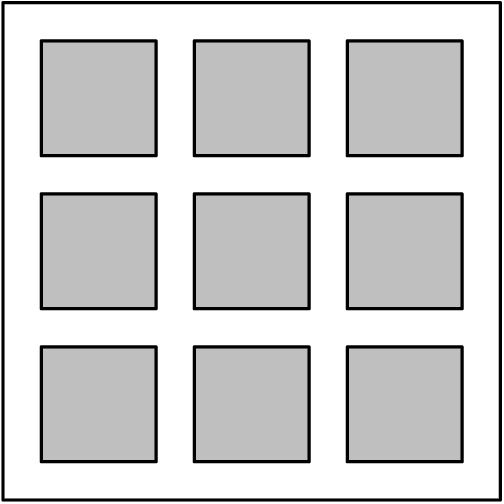
\includegraphics[height=0.3\textheight]{graytiles.png}
    \end{figure}
    (A) $\frac{6}{25}$ (B) $\frac{1}{4}$ (C) $\frac{9}{25}$ (D) $\frac{7}{16}$ (E) $\frac{9}{16}$
\end{frame}
\begin{frame}{Solution}
    注意到$n=24$时, 横行共有$25$个长为$d$的间隔, 共$24$个长为$s$的瓷砖边长, 因此我们有
    \begin{equation*}
        \frac{s^2\times 24^2}{(24s+25d)^2}=\frac{64}{100}
    \end{equation*}
    从而
    \begin{equation*}
        \frac{24^2}{(24+25d/s)^2}=\frac{64}{100}
    \end{equation*}
\end{frame}

% \begin{ques}
%     If $a$ and $b$ are integers such that $x^2-x-1$ is a factor of $ax^3+bx^2+1$, then $b$ is

%     如果$a$和$b$是整数,使得$x^2-x-1$是$ax^3+bx^2+1$的因子,求出$b$的值.

%     提示: 把$ax^3+bx^2+1$写成$(x^2-x-1)(cx+d),c\neq 0$, 然后展开对比两边的系数.
% \end{ques}
\begin{frame}{Homework}
    \begin{ques}[AMC 8, 2019-22]
        A store increased the original price of a shirt by a certain percent and then lowered the new price by the same amount. Given that the resulting price was $84 \%$ of the original price, by what percent was the price increased and decreased?
         (A) 16 (B) 20 (C) 28 (D) 36 (E) 40
    \end{ques}
    \begin{ques}
        Find the solution of the following equation:

        解下面的方程:
        \begin{itemize}
            \item $2x^2-9x=5$
            \item
                  \begin{equation*}
                      \frac{5}{x}+\frac{6}{x+1}=2
                  \end{equation*}
        \end{itemize}
    \end{ques}
\end{frame}
\begin{frame}{Homework}
    \begin{ques}
        For what values of the real number $k$ does $x^2+kx+4k=0$ have no real solutions.

        $k$取什么的时候$x^2+kx+4k=0$没有实根.
    \end{ques}
    \begin{ques}
        $x$是一个实数, 满足$|2x^2-9x+6|=2x^2-9x+6$, 求$x$的所有可能取值.
     \end{ques}
\end{frame}
\end{document}